\section{ТЕХНОЛОГИЯ ИССЛЕДОВАНИЯ}
На текущем этапе каждая из моделей дообучалась с оптимальными параметрами, а затем тестировалась. В качестве основных метрик для сравнения использовались accuracy, micro $F_1$ и macro $F_1$ на валидационных данных во время обучения. Кроме того, для выбора наиболее эффективной модели важно учитывать также данные о времени обучения, количестве занимаемой памяти во время обучения и количестве операций с плавающей точкой, затраченных на обучение моделей, а также скорость во время тестирования.

Все модели дообучались на 8 эпохах с ранней остановкой. Условие для ранней остановки: 
функция ошибки на валидационных данных не уменьшается в течение 3-х эпох.
\section{РЕЗУЛЬТАТЫ ИССЛЕДОВАНИЯ}
Проведя анализ графиков метрик во время обучения моделей 
(рисунок \ref{models-accuracy:image}, рисунок \ref{f1-macro:image}, рисунок \ref{f1-micro:image}) можно сделать вывод, что наиболее точной 
моделью является RoBERTa, тогда как наименее точной моделью оказался BERT. Однако стоит отметить, что точность моделей отличается незначительно 
(около 1\%). 
\begin{figure}[H]
   \begin{center}
      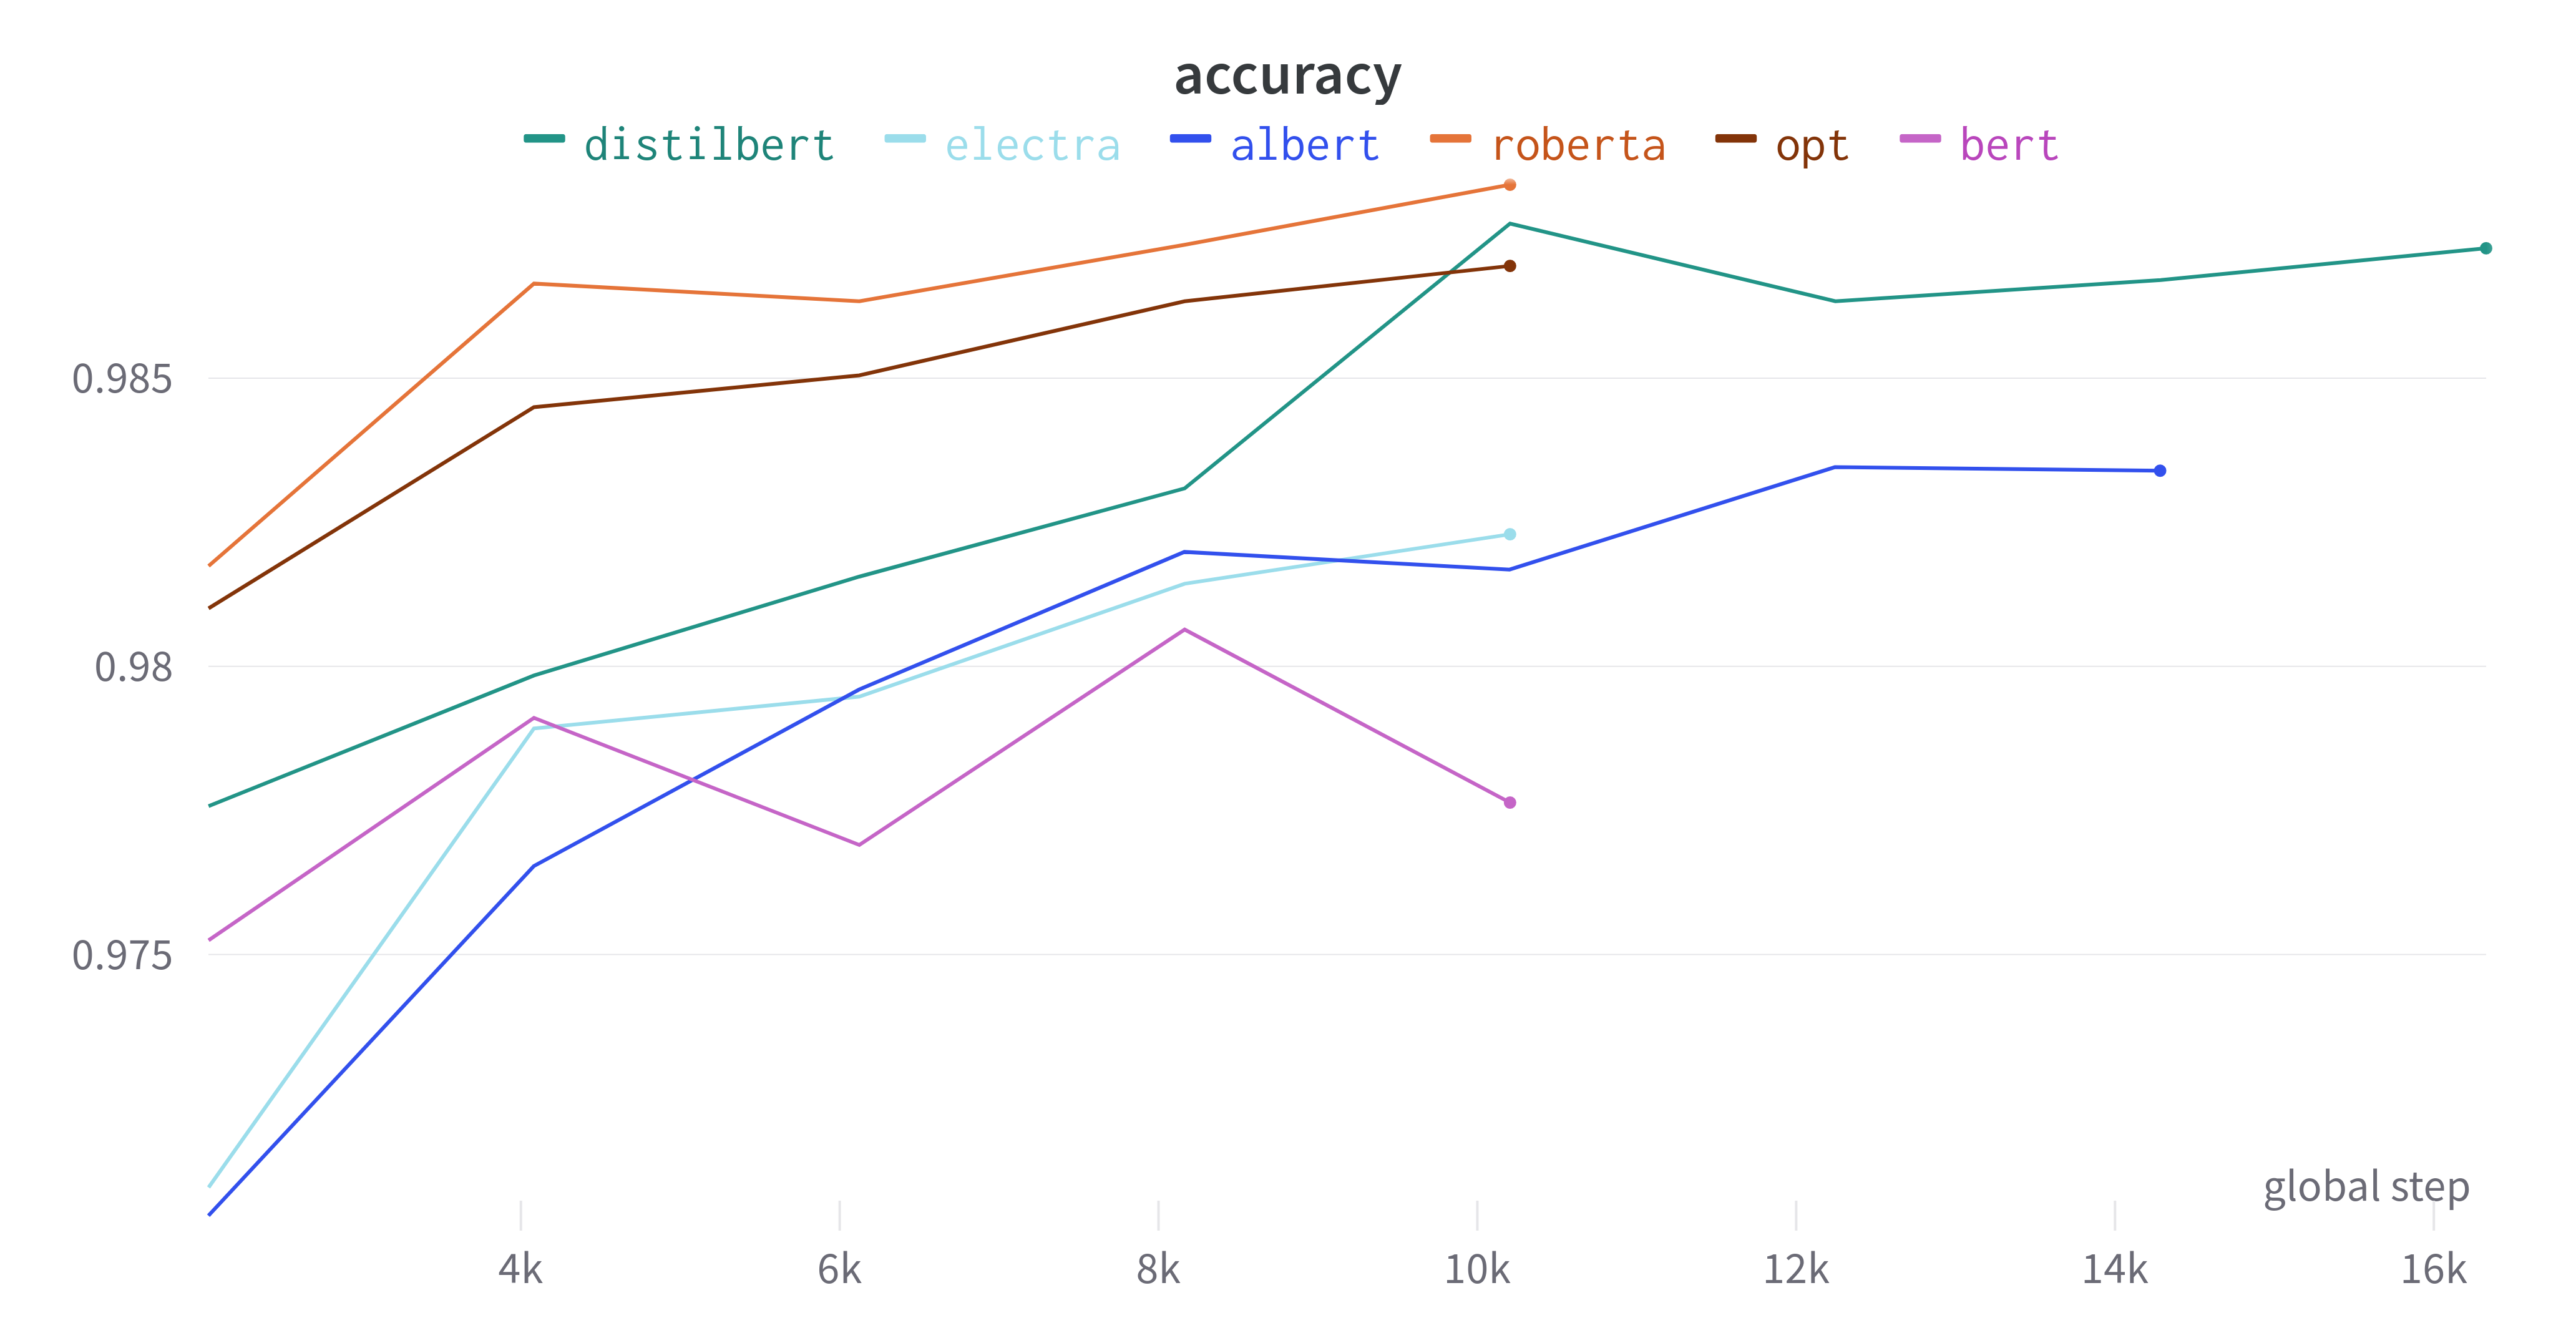
\includegraphics[width=.7\linewidth]{models/accuracy.png}
      \caption{График точности во время обучения моделей}
      \label{models-accuracy:image}
   \end{center}
\end{figure}

\begin{figure}[H]
   \begin{center}
      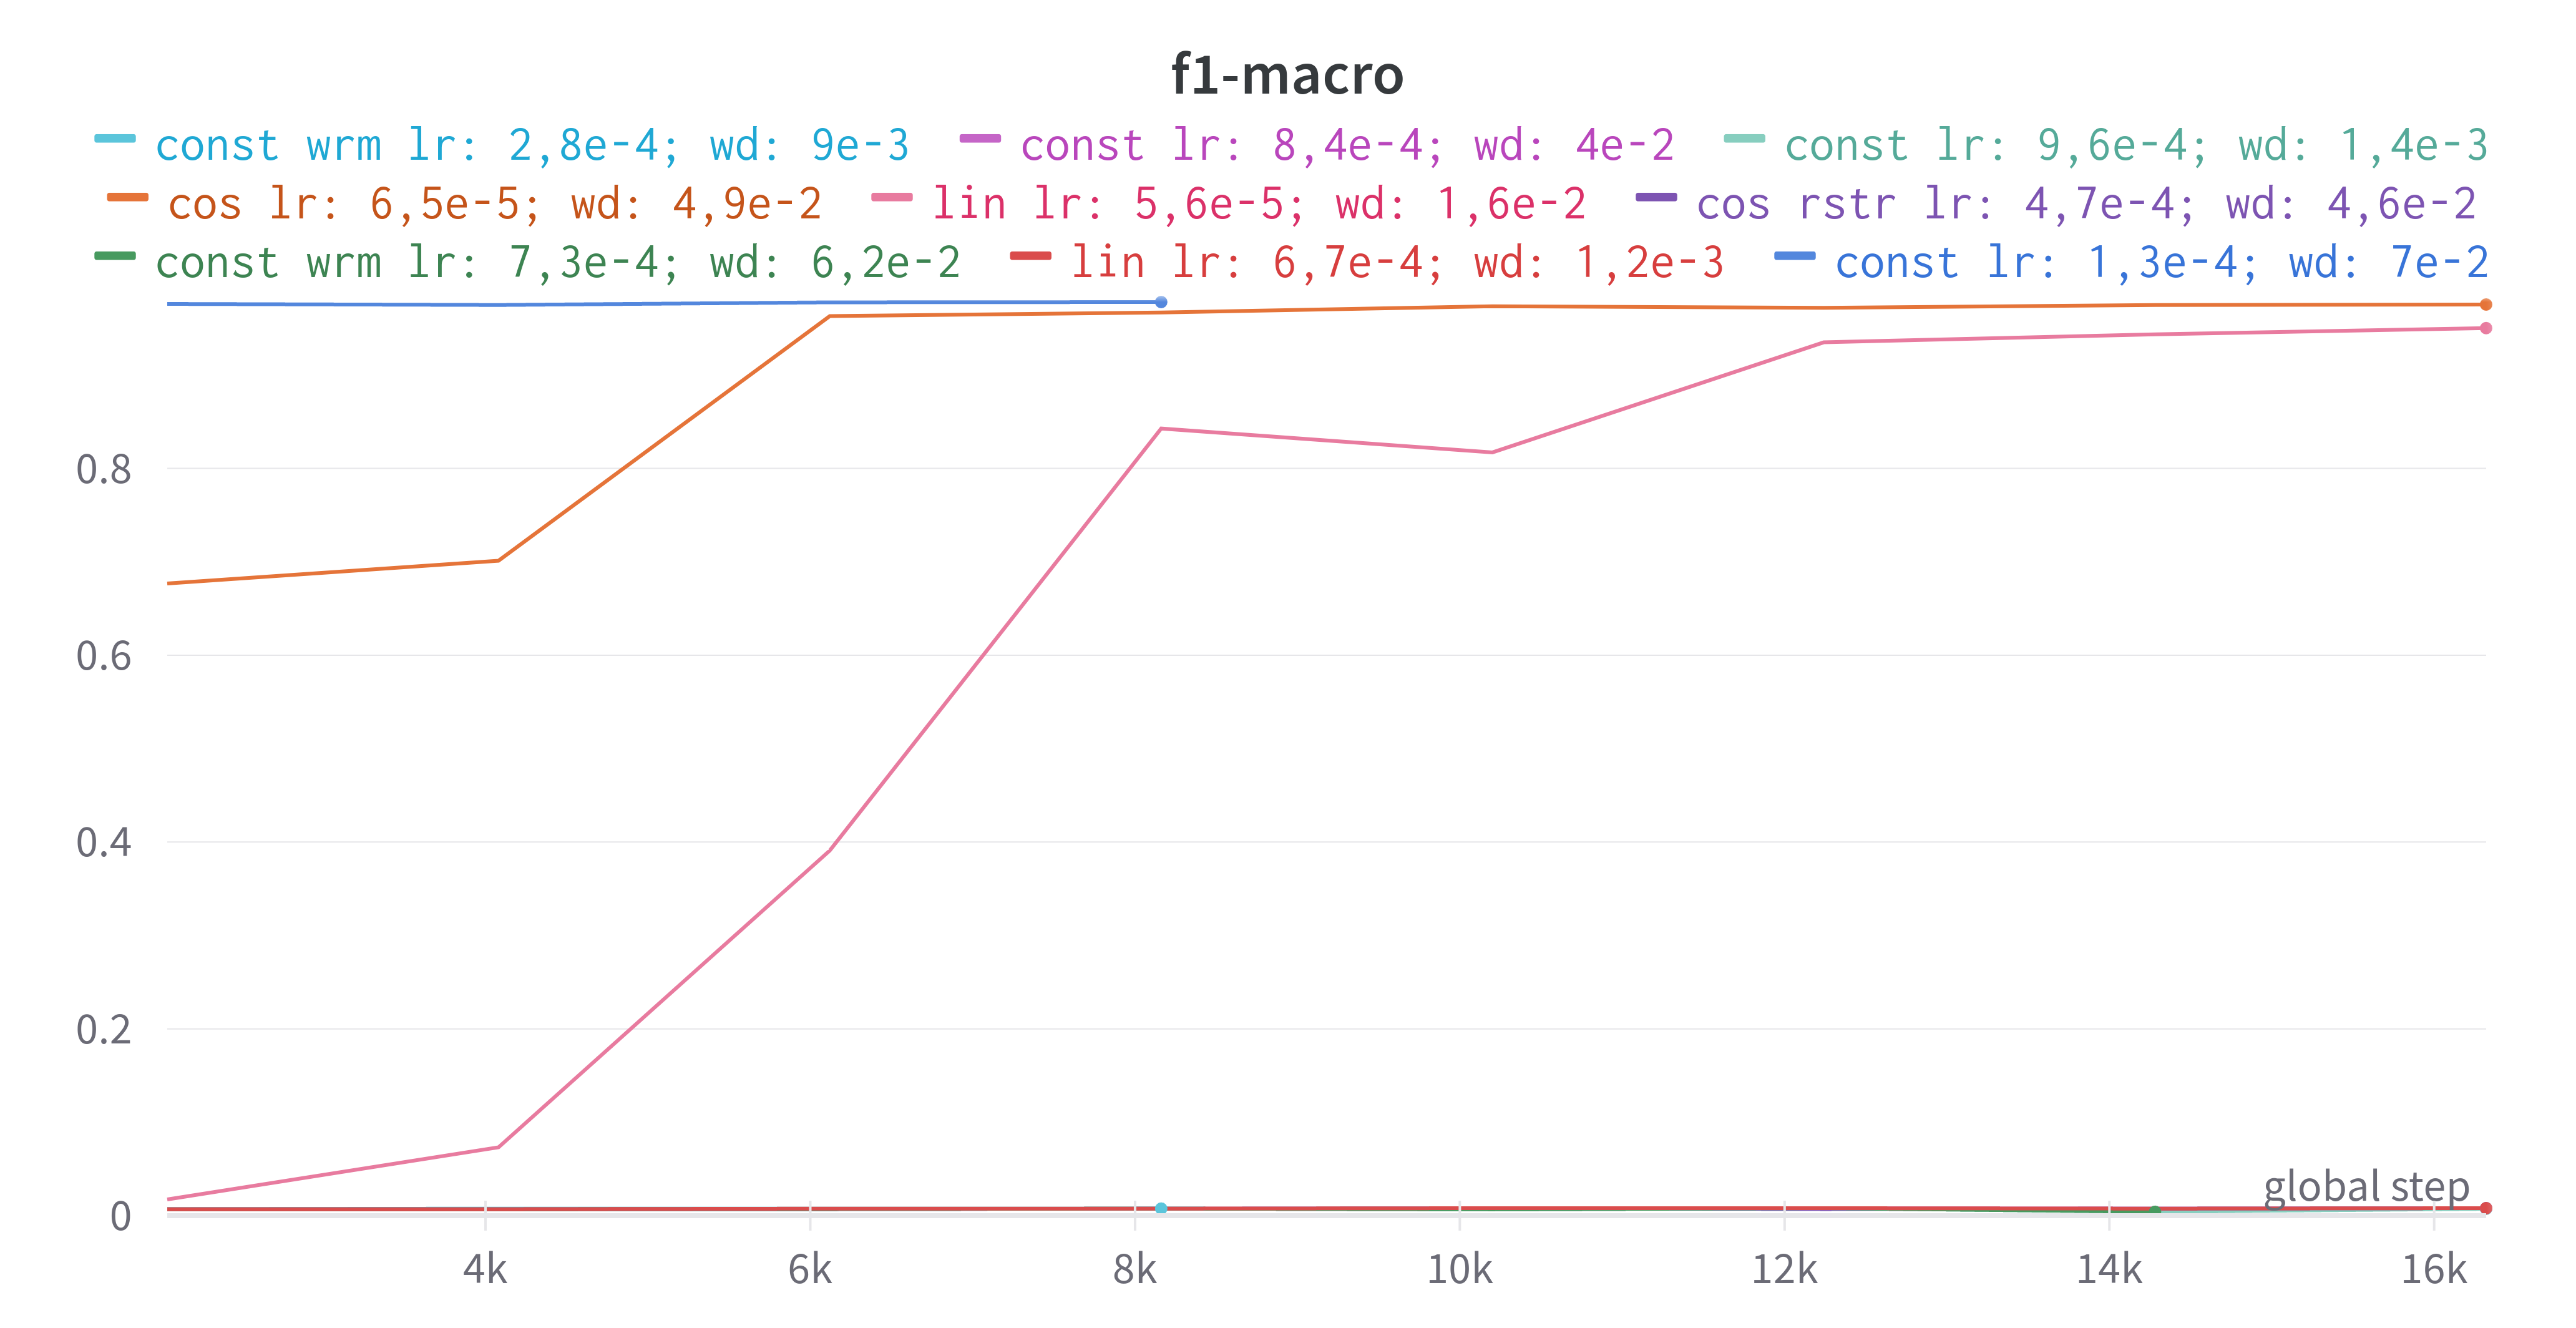
\includegraphics[width=.9\linewidth]{models/f1-macro.png}
      \caption{График macro $F_1$ во время обучения моделей}
      \label{f1-macro:image}
   \end{center}
\end{figure}

\begin{figure}[H]
   \begin{center} 
      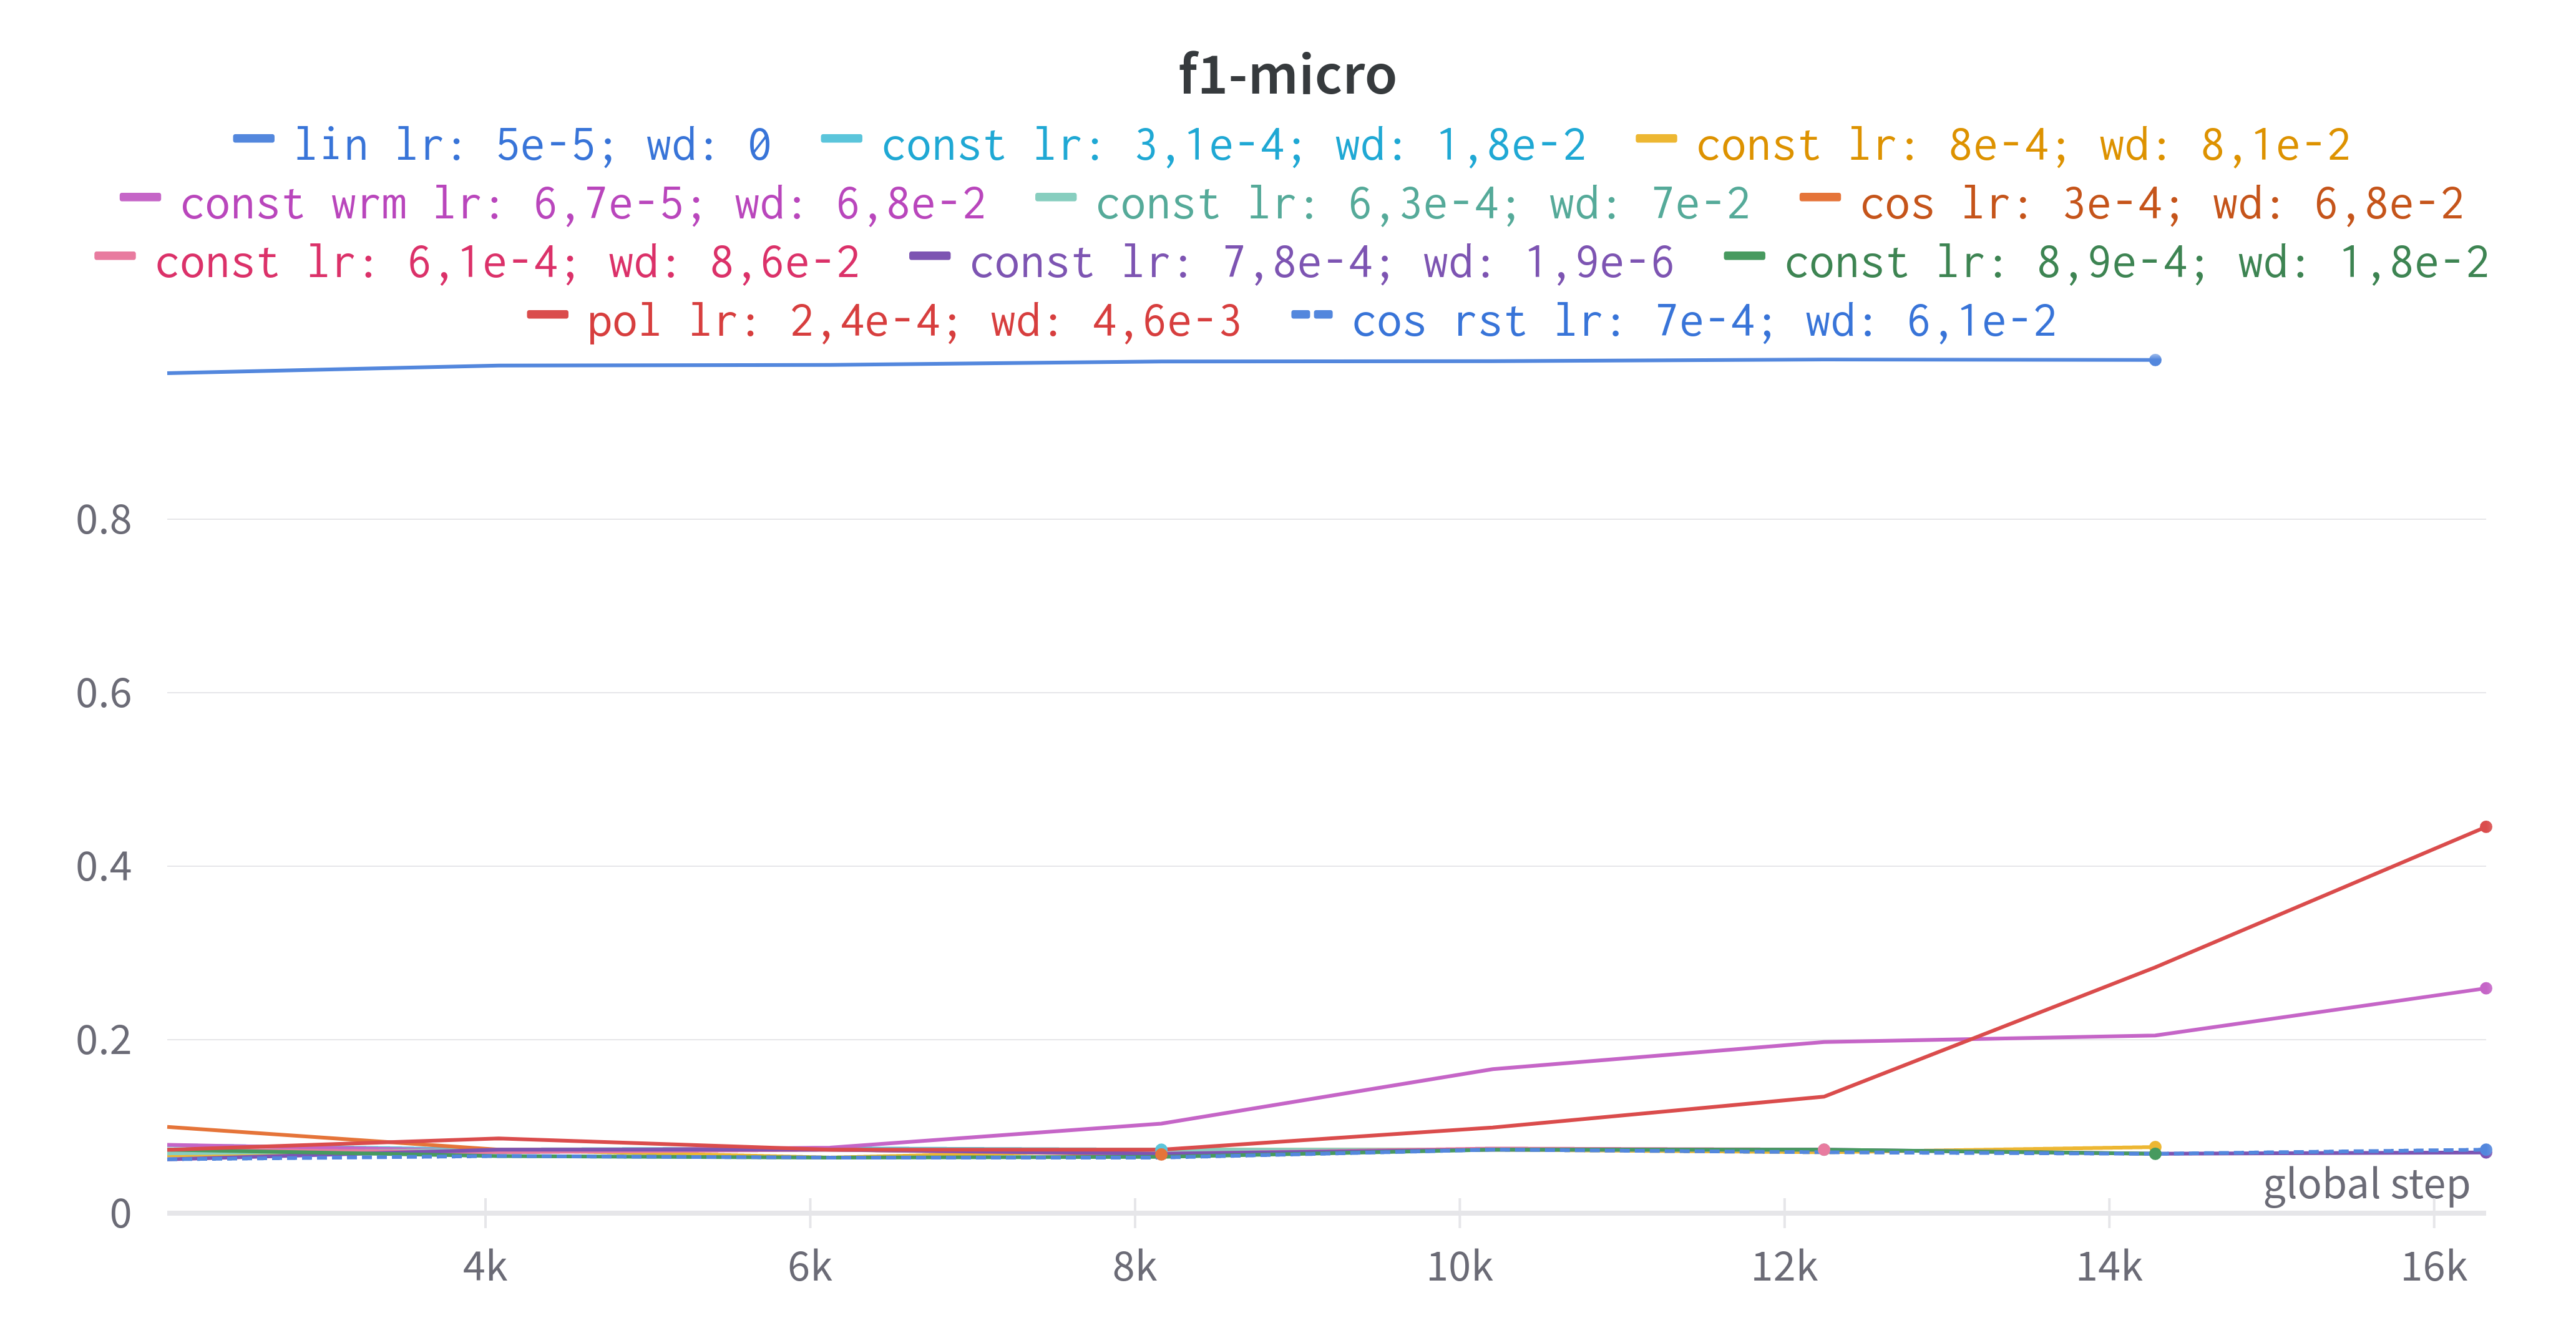
\includegraphics[width=.9\linewidth]{models/f1-micro.png}
      \caption{График micro $F_1$ во время обучения моделей}
      \label{f1-micro:image}
   \end{center} 
\end{figure}

По количеству занимаемой памяти и скорости обучения (рисунок \ref{gpu-memory:image}, рисунок \ref{train-runtime:image}) RoBERTa 
также является лучшей моделью. По количеству операций с плавающей точкой, затраченных на обучение 
(рисунок \ref{flos:image}), RoBERTa уступает лишь ALBERT и ELECTRA.  

\begin{figure}[H]
   \begin{center}
      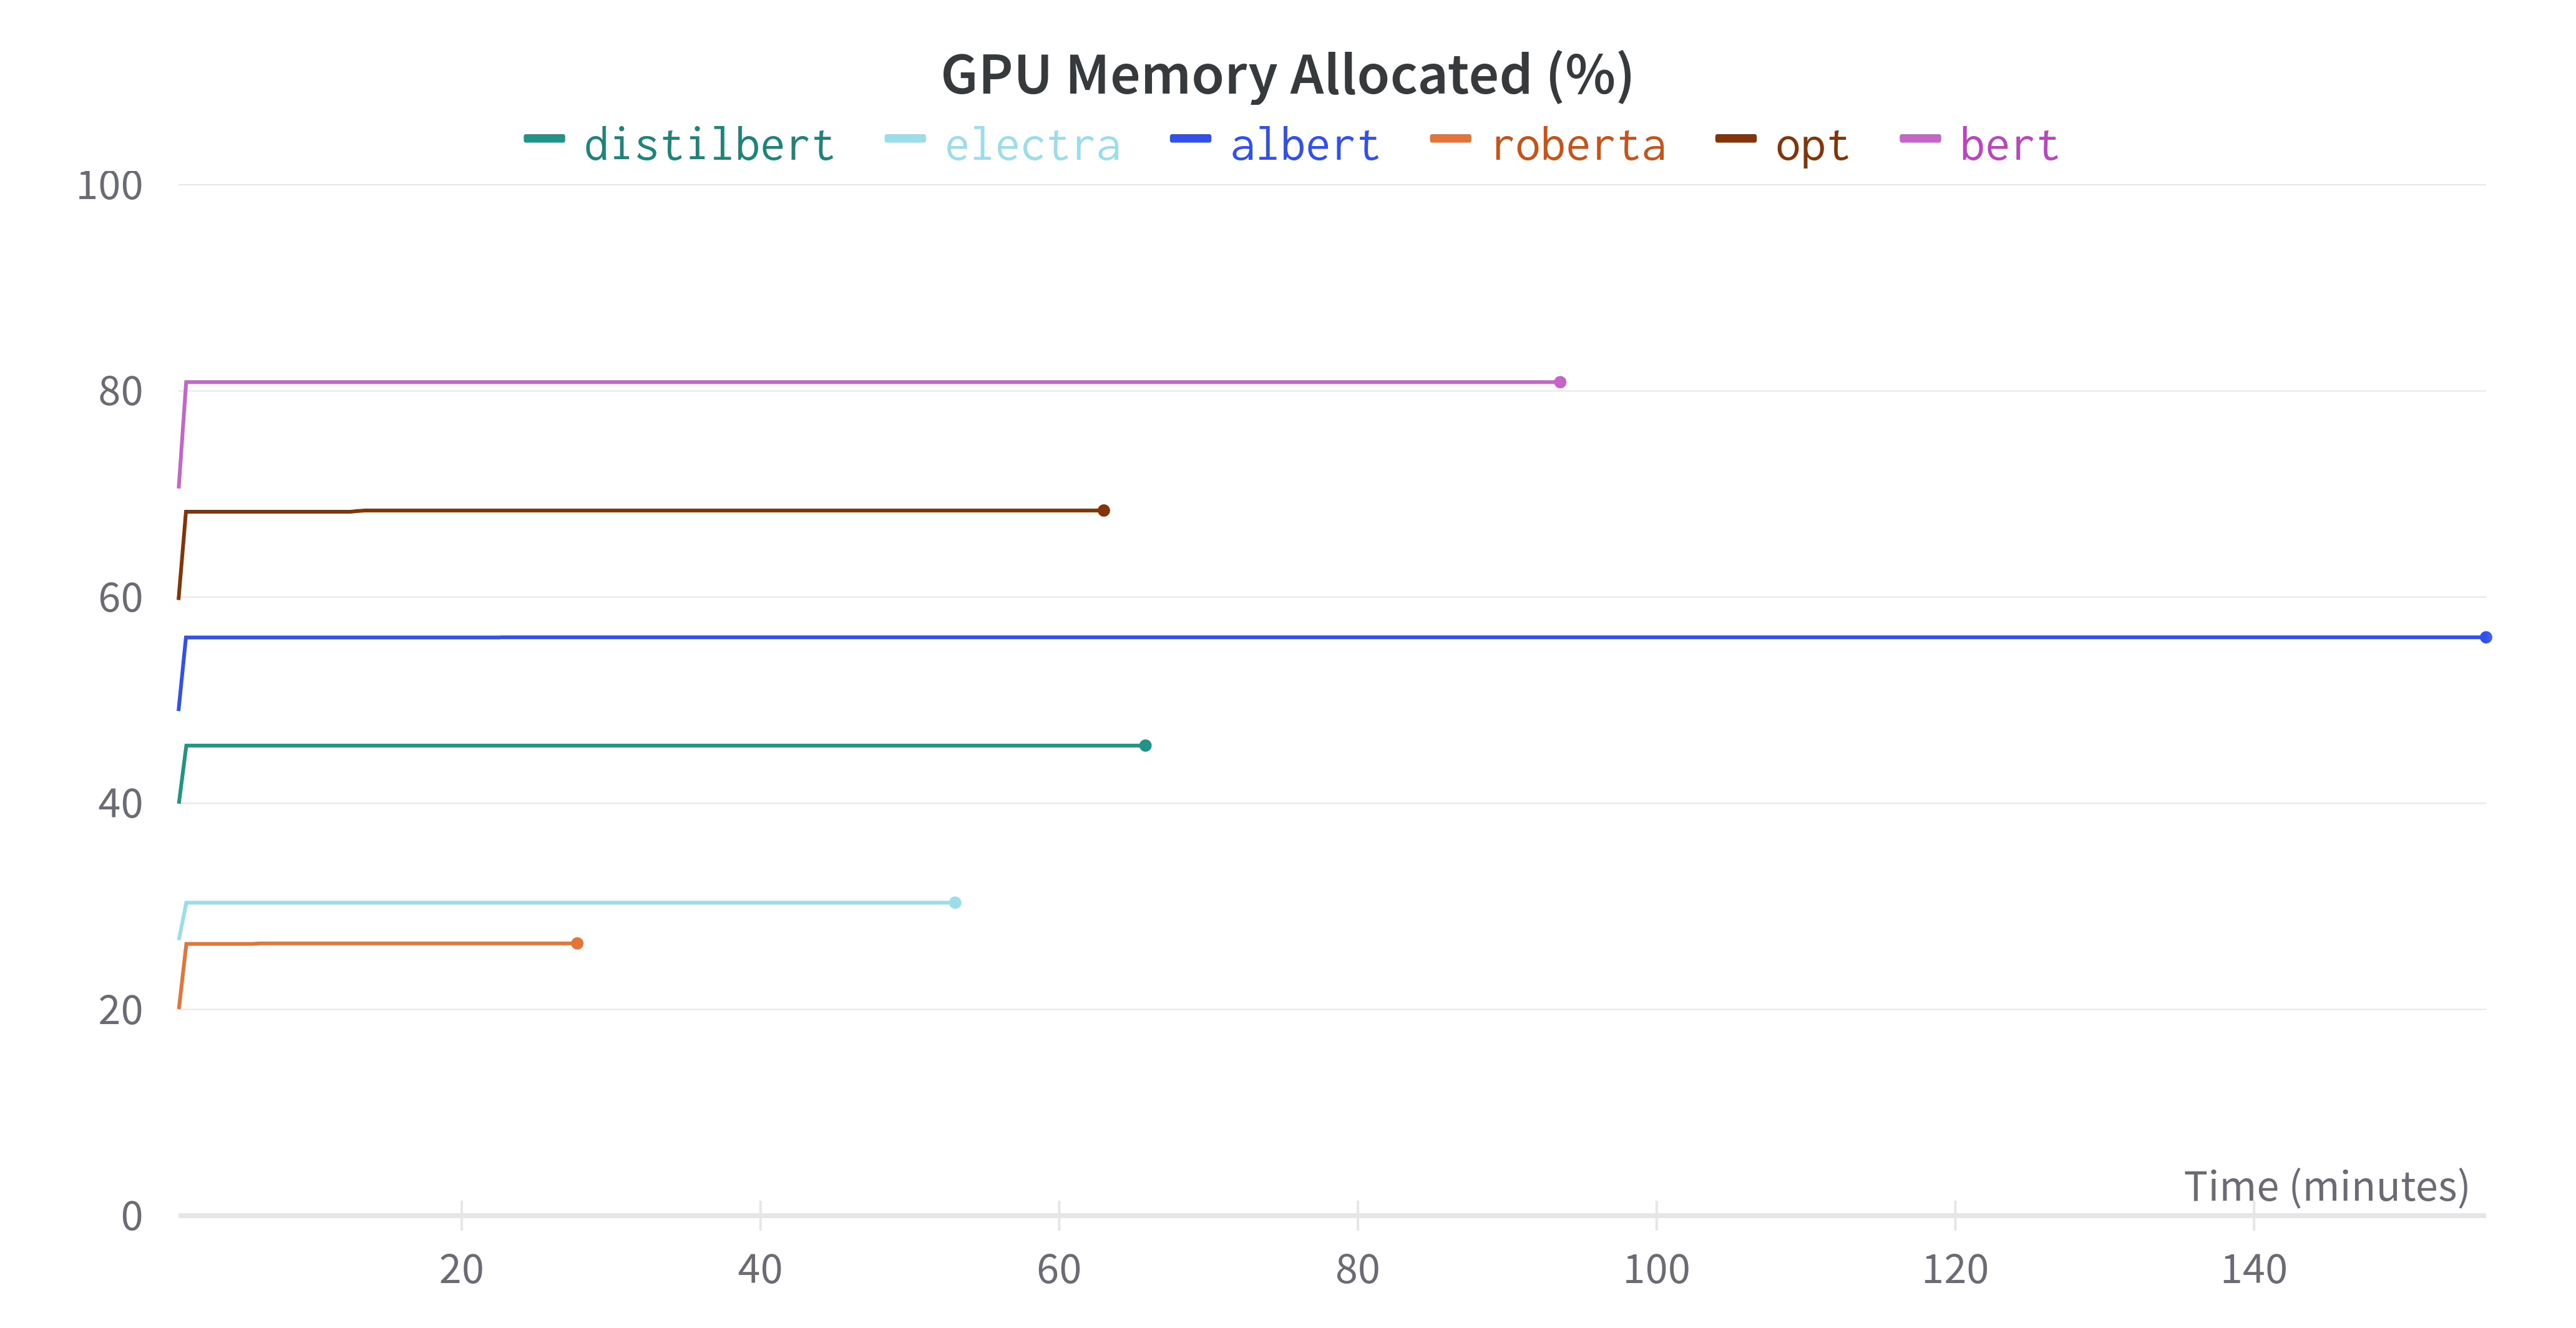
\includegraphics[width=\linewidth]{models/gpu-memory.png}
      \caption{Процент видеопамяти, занимаемый моделью при обучении}
      \label{gpu-memory:image}
   \end{center}
\end{figure}

\begin{figure}[H]
   \begin{center}
      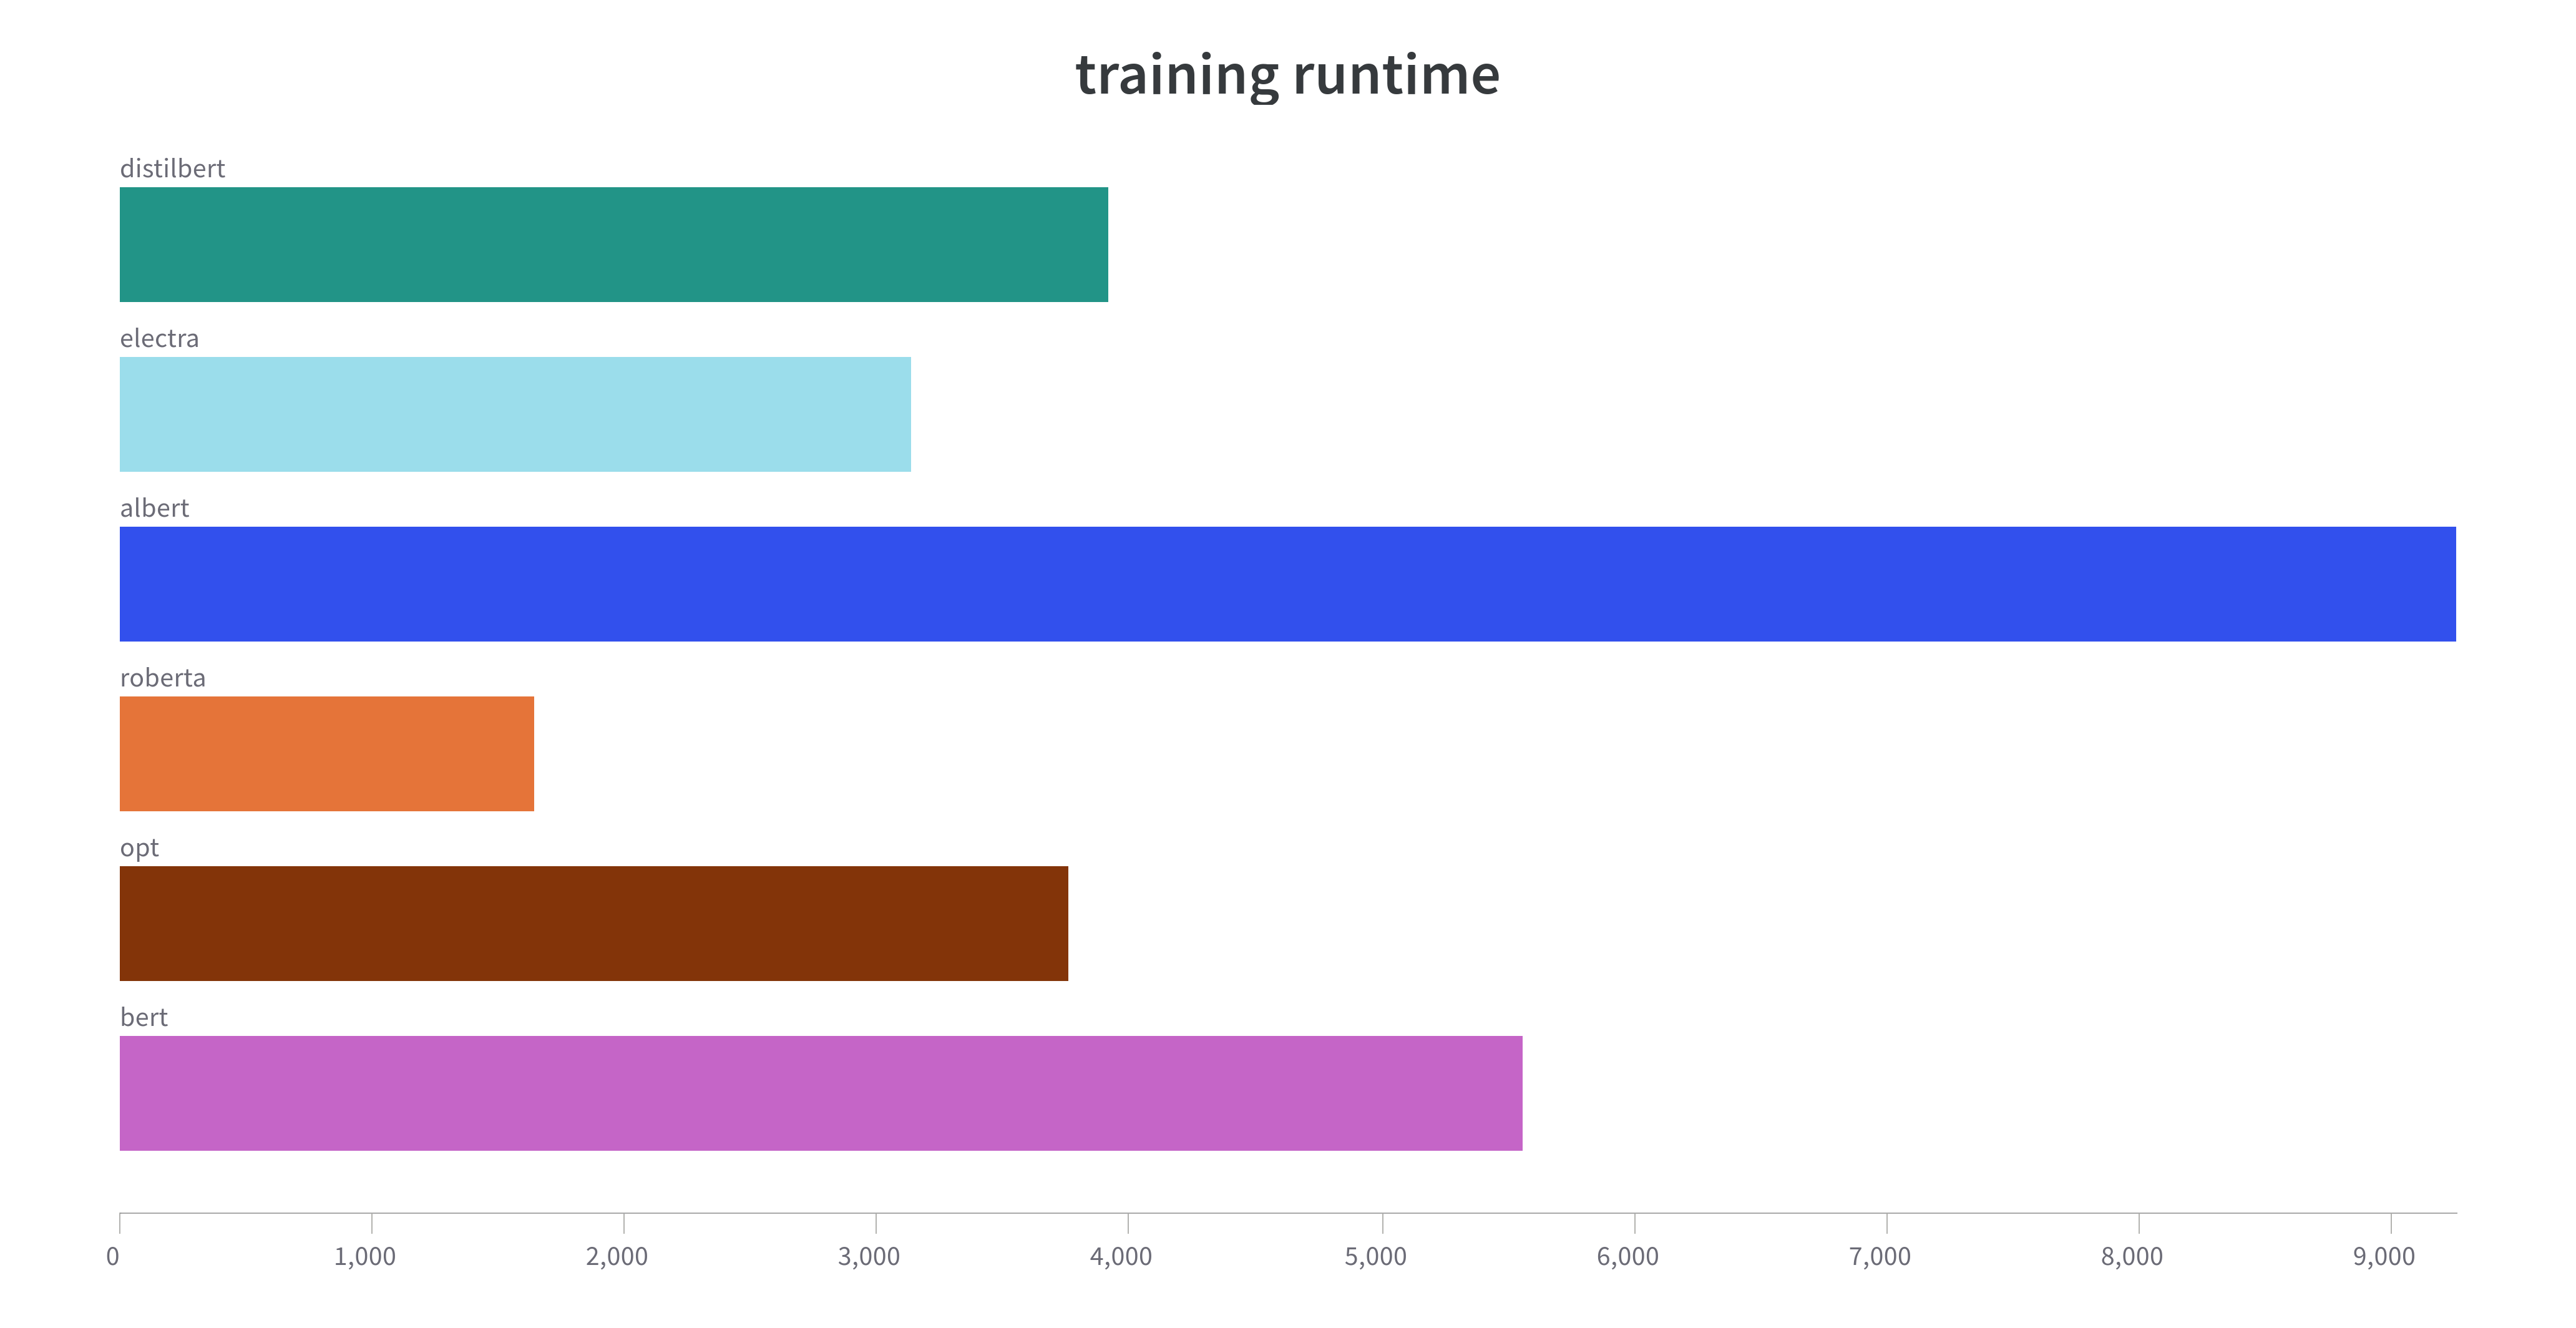
\includegraphics[width=\linewidth]{models/train-runtime.png}
      \caption{Время, затраченное на обучение}
      \label{train-runtime:image}
   \end{center}
\end{figure}

\begin{figure}[H]
   \begin{center}
      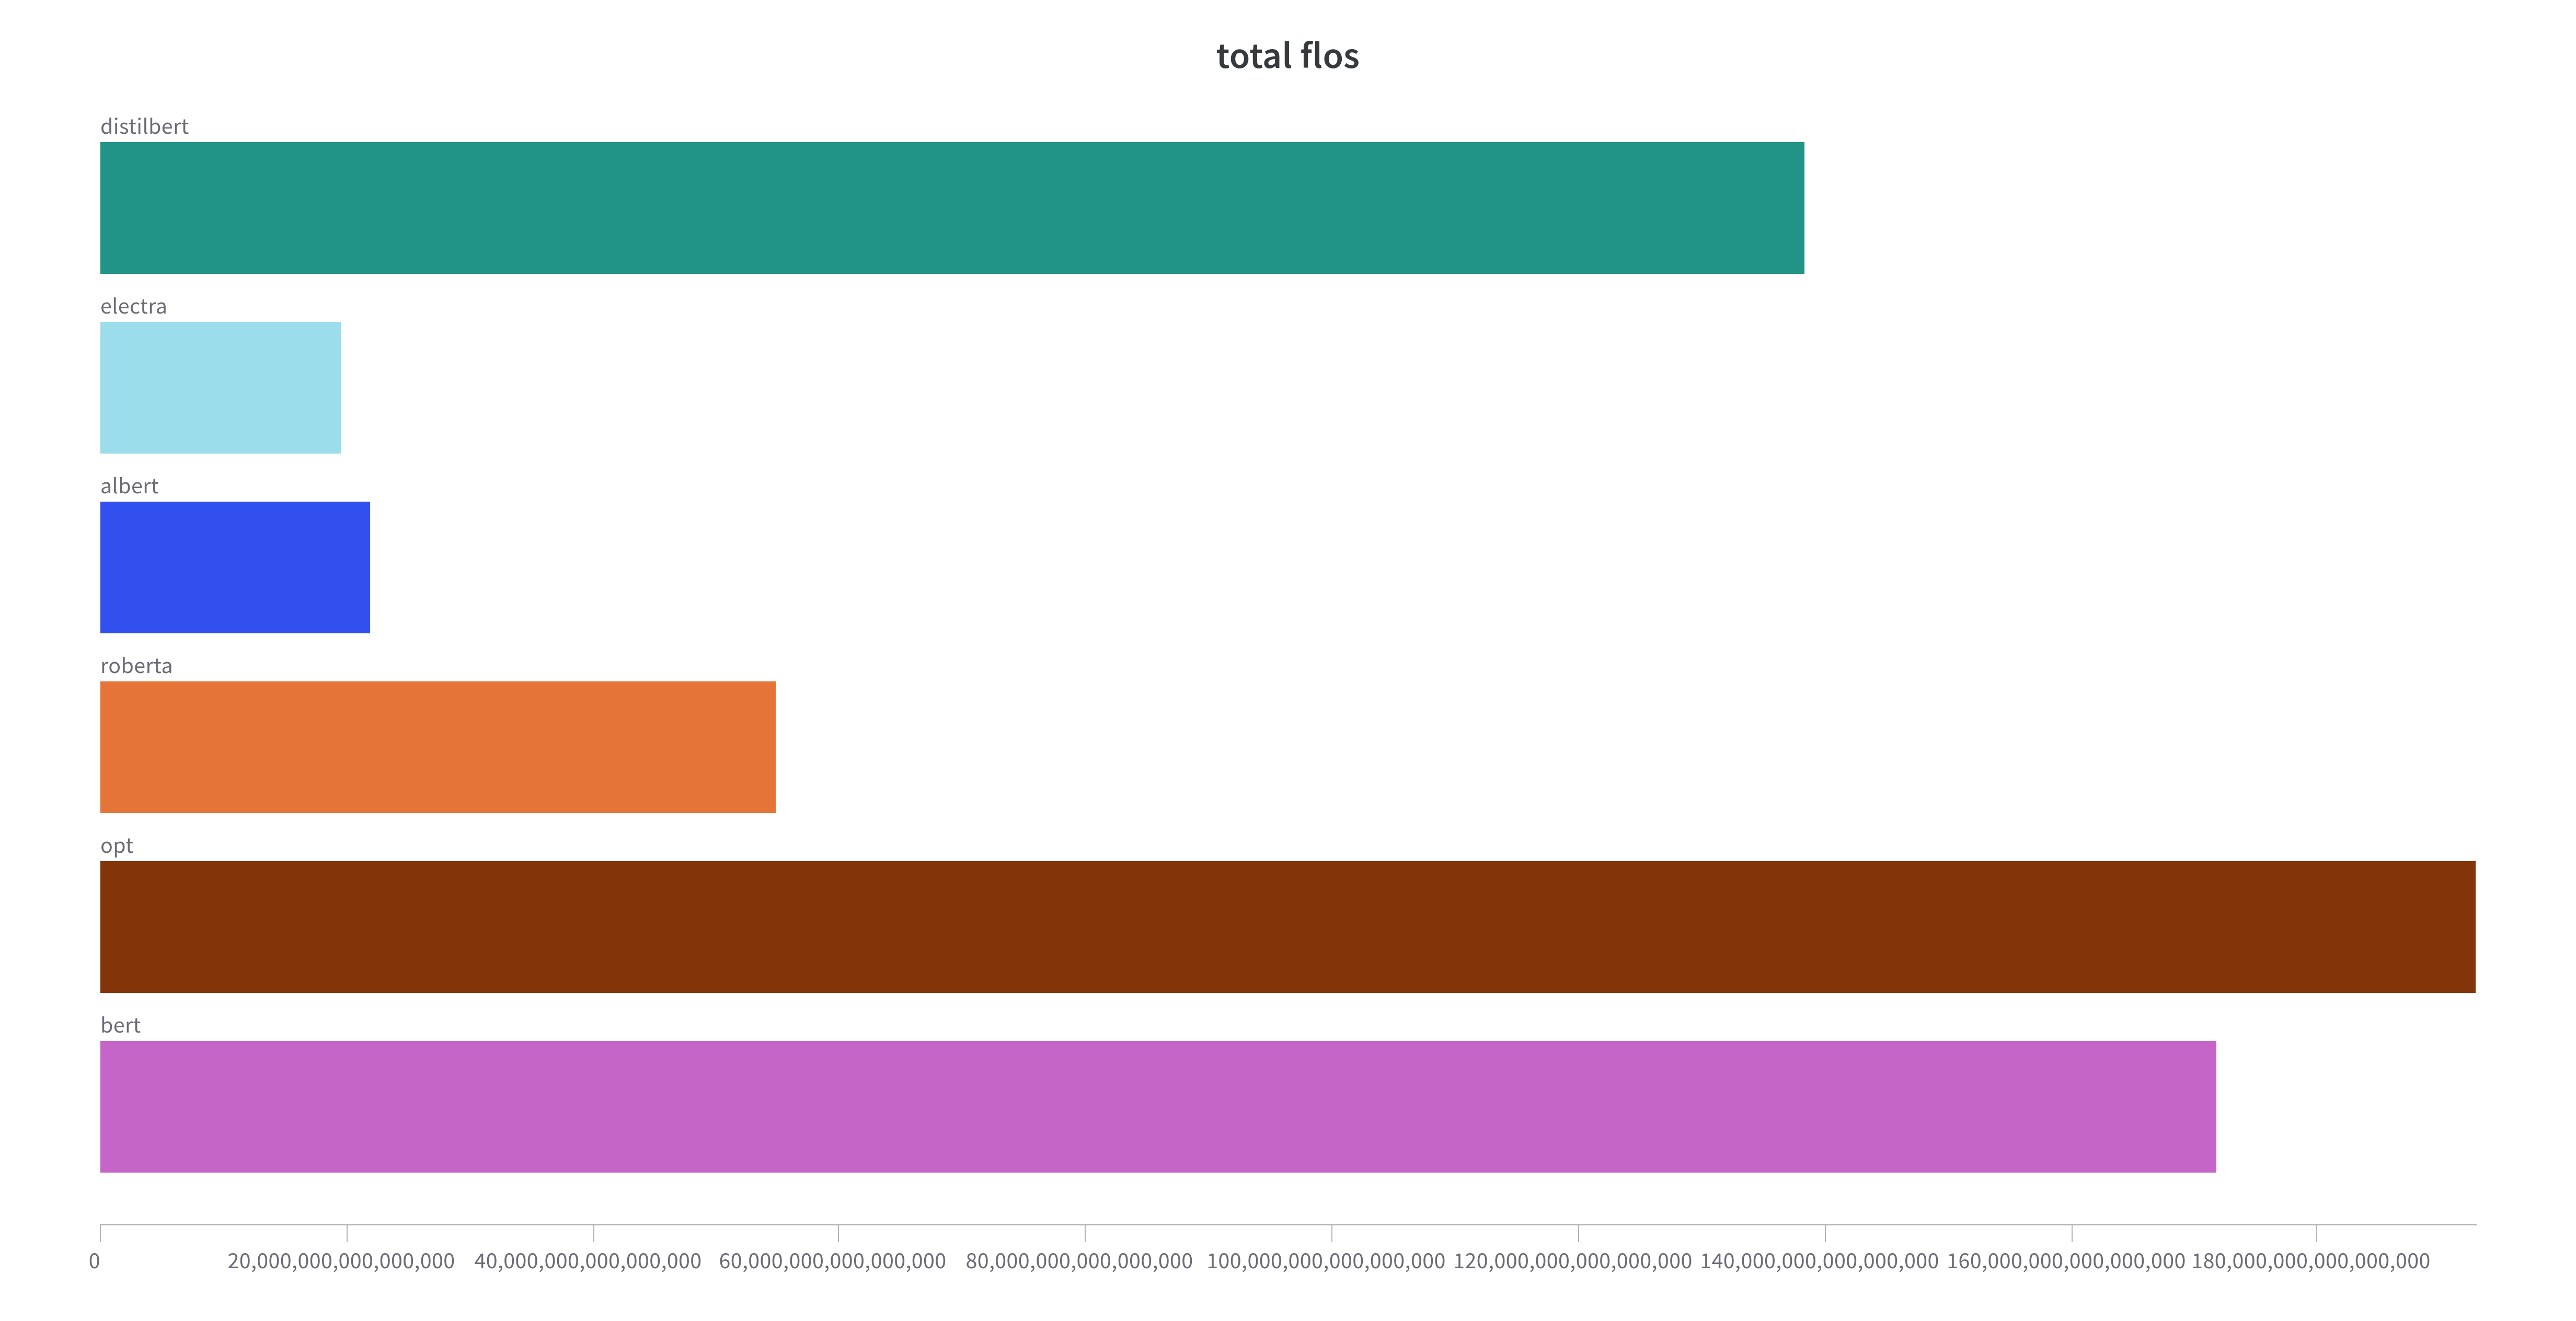
\includegraphics[width=\linewidth]{models/flos.png}
      \caption{Количество операций с плавающей точкой, затраченных на обучение}
      \label{flos:image}
   \end{center}
\end{figure}

По скорости при использовании (рисунок \ref{test-runtime:image}, рисунок \ref{test-samples:image}) RoBERTa также является наиболее оптимальной моделью. 

%\begin{figure}[H]
%   \begin{center}
%      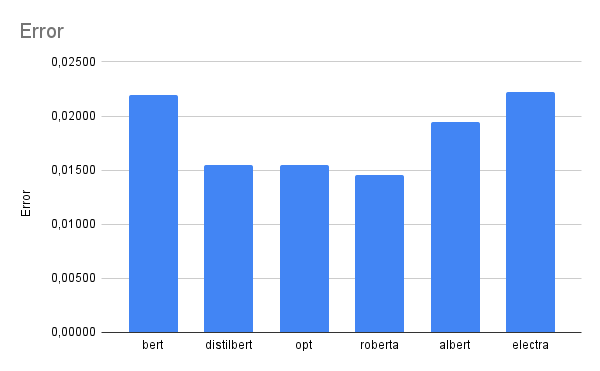
\includegraphics[width=.9\linewidth]{test/error.png}
%      \caption{Ошибка на тестовых данных}
%      \label{test-accuracy:image}
%   \end{center}
%\end{figure}

%\begin{figure}[H]
%   \begin{center}
%      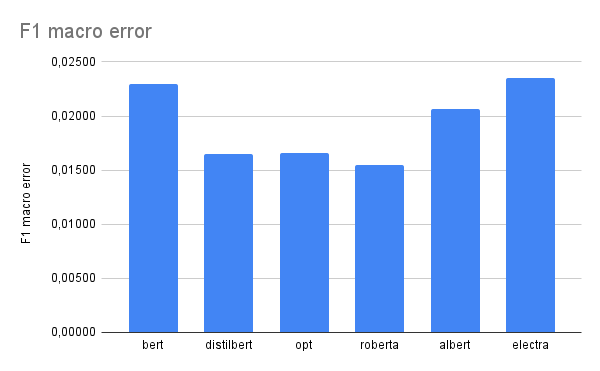
\includegraphics[width=.9\linewidth]{test/f1-macro-error.png}
%      \caption{Ошибка macro $F_1$ на тестовых данных}
%      \label{test-f1-macro:image}
%   \end{center}
%\end{figure}

%\begin{figure}[H]
%   \begin{center}
%      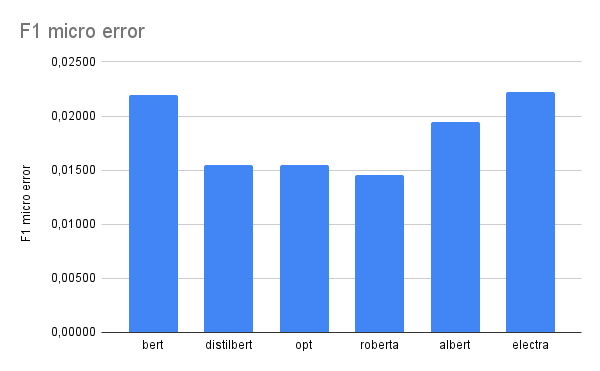
\includegraphics[width=.9\linewidth]{test/f1-micro-error.png}
%      \caption{Ошибка micro $F_1$ на тестовых данных}
%      \label{test-f1-micro:image} 
%   \end{center}
%\end{figure}

\begin{figure}[H]
   \begin{center}
      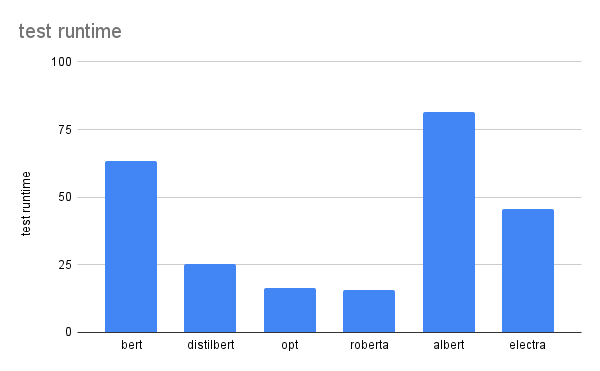
\includegraphics[width=.9\linewidth]{test/test runtime.png}
      \caption{Время, затраченное на тестирование}
      \label{test-runtime:image}
   \end{center}
\end{figure}

\begin{figure}[H]
   \begin{center}
      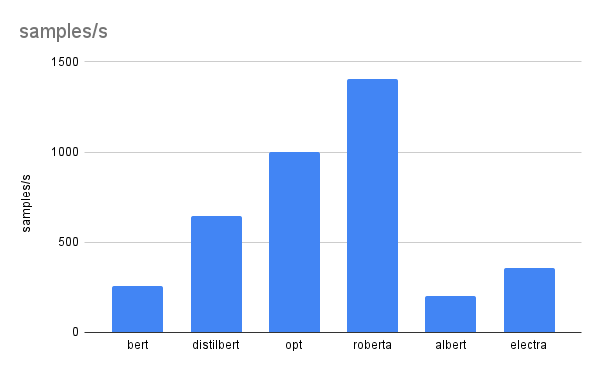
\includegraphics[width=.9\linewidth]{test/samples_s.png}
      \caption{Скорость при тестировании}
      \label{test-samples:image}
   \end{center}
\end{figure}

График функции ошибки во время обучения и график функции ошибки на валидационных данных можно 
найти в приложении \ref{app:models}.

\section{ТЕСТИРОВАНИЕ И ПРИМЕРЫ РАБОТЫ ИТОГОВОЙ МОДЕЛИ}
Проанализировав метрики на тестовых данных (таблица \ref{test-metrics:table}) и примеры работы итоговой модели выделения интентов (таблица \ref{test-examples:table}) можно сделать вывод, что модель неплохо справляется с поставленной задачей, однако наличие неправильно классифицированных интентов может говорить о неполноте данных и сложности в различении некоторых интентов. Например, вопросы <<Как дела?>> или <<Что нового?>> в английском языке могут использоваться в качестве приветствия. Отдельной проблемой является распознавание шуток. Это требует дальнейшей работы над обучающим набором данных для улучшения итогового результата.
\begin{table}[H]
   \captionsetup{format=hang, singlelinecheck=false}
   \raggedleft
      \caption{Метрики на тестовых данных}
      \label{test-metrics:table}
   \centering        
   \begin{tabular}{|p{4cm}|p{4cm}|}
      \hline
      Accuracy & 98,54\% \\
      \hline
      Micro $F_1$ & 98,54\% \\
      \hline
      Macro $F_1$ & 98,45\% \\
      \hline
   \end{tabular}
\end{table}

\begin{table}[H]
   \captionsetup{format=hang, singlelinecheck=false}
   \raggedleft
      \caption{Примеры работы итоговой модели}
      \label{test-examples:table}
   \centering        
   \begin{tabular}{|p{8cm}|p{8cm}|}
      \hline
      Примеры & Предсказанные классы примеров \\
      \hline
      Hello, Jack! & Greeting \\
      \hline
      I want you to attack that people. & Attack \\
      \hline
      Can i buy something from you? & Exchange \\
      \hline
      1234 & Drival \\
      \hline
      Is here job for me? & Receive quest \\
      \hline
      I'm going to hurt you! & Threat \\
      \hline
      Can you deliver this message to capital? & Message \\
      \hline
      What can you tell me about this lands? & Knowledge \\
      \hline
      Goodbye, my friend! & Farewell \\
      \hline
      fight can low be common & Drival \\
      \hline
      Follow me. & Follow \\
      \hline
      How are you today? & Greeting \\
      \hline
      What are you doing today? & Greeting \\
      \hline
      How are you today? & Greeting \\
      \hline
      What are you doing here? & Knowledge \\
      \hline
      Can you help me? & Join \\
      \hline
      Why is the chicken crossing the road? & Knowledge \\
      \hline
   \end{tabular}
\end{table}
